\section{Experiments}
\label{sec:experiments}

\subsection{Experimental Setup}
\label{sec:experimental_setup}

\vspace{-0.5em}
\paragraph{Datasets.}
We evaluate \name in two complementary settings: tool-integrated reasoning and long-horizon agentic tasks.
For tool-integrated reasoning, the training set contains 34,501 prompts drawn from 14,116 examples from the English subset of DAPO-Math, 10,385 examples from the code subset of Skywork-OR1-RL-Data, and 10,000 examples from MegaScience~\citep{abs-2503-14476,abs-2505-22312,abs-2507-16812}. 
We evaluate mathematical reasoning on AIME 2024--2026 and HMMT February 2026~\citep{aime24,aime25,aime26,abs-2605-00674}, scientific reasoning on GPQA~\citep{abs-2311-12022}, and code generation on LiveCodeBench v6~\citep{JainHGLYZWSSS25}.
For long-horizon interaction, we train and evaluate on the official splits of ALFWorld~\citep{ShridharYCBTH21} and ScienceWorld~\citep{WangJCA22}.
Both environments require the agent to condition successive actions on environment feedback, which makes them a direct test of robustness to compounding inter-turn error.

\vspace{-0.5em}
\paragraph{Baselines.}
We compare \name with the original student checkpoint (\textsc{Vanilla}), standard \textsc{OPD}~\citep{AgarwalVZSGGB24,Gu0WH24}, and five OPD methods that improve training stability through selective guidance or curricula: \textsc{SAGE-OPD}~\citep{abs-2606-19659}, \textsc{Guided-OPD}~\citep{abs-2606-15912}, \textsc{Relay-OPD}~\citep{abs-2607-26057}, \textsc{TCOD}~\citep{abs-2604-24005}, and \textsc{FutureBridge-OPD}~\citep{abs-2608-01953}.
All distillation methods share the same teacher and student initializations, prompts, rollout budget, and evaluation protocol, so the main comparison controls for differences in data and rollout configuration.
We additionally provide a comparison under a matched teacher-intervention budget in \Cref{app:teacher_computation_matched}.

\vspace{-0.5em}
\paragraph{Implementation Details.}
We use Qwen3-0.6B and Qwen3-1.7B as students and Qwen3-4B as the teacher~\citep{abs-2505-09388} and additional experiments with Qwen3-32B examine scaling to a stronger teacher.
Evaluation uses the student policy alone, with no teacher intervention.
All reported numbers are means over multiple independent runs (refer to the detailed experimental results), and the reported uncertainties are standard deviations across those runs. 
Complete hyperparameters and prompts are given in \Cref{app:training_parameters,app:prompts}. 

\begin{table}[t]
\centering 
\caption{Results on tool-integrated reasoning benchmarks. Bold and underlined values denote the best and second-best results, respectively.}
\label{tab:tir_results}
\resizebox{1.\linewidth}{!}{
\begin{tabular}{lcccccc}
\toprule
\multirow{2}{*}{\textbf{Method}} & \cellcolor{cyan!20} \textbf{AIME24} & \cellcolor{cyan!20} \textbf{AIME25} & \cellcolor{cyan!20} \textbf{AIME26} & \cellcolor{cyan!20} \textbf{HMMT26} & \cellcolor{Orchid!20} \textbf{GPQA} & \cellcolor{LimeGreen!20} \textbf{LiveCodeBench v6} \\
& \multicolumn{4}{c}{\cellcolor{cyan!20} \textbf{Avg@32}} & \multicolumn{1}{c}{\cellcolor{Orchid!20} \textbf{Avg@8}} & \multicolumn{1}{c}{\cellcolor{LimeGreen!20} \textbf{Avg@8}} \\
\midrule 
\multicolumn{7}{c}{\cellcolor{gray!10} \textit{\textbf{Qwen3-4B}}} \\
\textsc{Teacher} & $71.7_{\pm 0.3}$ & $65.0_{\pm 0.3}$ & $60.0_{\pm 0.3}$ & $39.8_{\pm 0.3}$ & $50.9_{\pm 0.3}$ & $70.5_{\pm 0.3}$ \\
\midrule
\multicolumn{7}{c}{\cellcolor{gray!10} \textit{\textbf{Qwen3-0.6B}}} \\
\textsc{Vanilla} & $8.3_{\pm 0.4}$ & $15.8_{\pm 0.6}$ & $9.6_{\pm 0.5}$ & $10.2_{\pm 0.4}$ & $26.0_{\pm 0.7}$ & $20.7_{\pm 0.5}$ \\
\textsc{OPD} & $11.2_{\pm 0.5}$ & $18.5_{\pm 0.5}$ & $12.4_{\pm 0.4}$ & $11.8_{\pm 0.6}$ & $27.1_{\pm 0.6}$ & $23.5_{\pm 0.7}$ \\
\textsc{SAGE-OPD} & $14.5_{\pm 0.6}$ & $21.0_{\pm 0.7}$ & $14.8_{\pm 0.6}$ & $13.9_{\pm 0.5}$ & $28.6_{\pm 0.5}$ & $26.2_{\pm 0.6}$ \\
\textsc{Guided-OPD} & $18.2_{\pm 0.7}$ & $25.1_{\pm 0.6}$ & $17.5_{\pm 0.7}$ & $16.2_{\pm 0.5}$ & $29.8_{\pm 0.6}$ & $31.4_{\pm 0.8}$ \\
\textsc{Relay-OPD} & $16.8_{\pm 0.5}$ & $23.4_{\pm 0.8}$ & $16.1_{\pm 0.5}$ & $14.7_{\pm 0.6}$ & $28.2_{\pm 0.7}$ & $29.1_{\pm 0.7}$ \\
\textsc{TCOD} & $20.4_{\pm 0.8}$ & $27.9_{\pm 0.7}$ & $19.3_{\pm 0.6}$ & $15.8_{\pm 0.7}$ & \underline{$31.2_{\pm 0.6}$} & $33.6_{\pm 0.8}$ \\
\textsc{FutureBridge-OPD} & \underline{$22.1_{\pm 0.7}$} & \underline{$30.2_{\pm 0.8}$} & \underline{$20.8_{\pm 0.7}$} & \underline{$17.5_{\pm 0.5}$} & $30.9_{\pm 0.5}$ & \underline{$35.8_{\pm 0.9}$} \\
\midrule
\name & \textbf{24.2}$_{\pm \mathbf{0.4}}$ & \textbf{33.5}$_{\pm \mathbf{0.4}}$ & \textbf{22.7}$_{\pm \mathbf{0.3}}$ & \textbf{18.6}$_{\pm \mathbf{0.3}}$ & \textbf{32.5}$_{\pm \mathbf{0.3}}$ & \textbf{38.8}$_{\pm \mathbf{0.4}}$ \\
\midrule
\multicolumn{7}{c}{\cellcolor{gray!10} \textit{\textbf{Qwen3-1.7B}}} \\
\textsc{Vanilla} & $42.9_{\pm 0.6}$ & $35.8_{\pm 0.7}$ & $32.8_{\pm 0.5}$ & $25.0_{\pm 0.6}$ & $34.2_{\pm 0.8}$ & $44.1_{\pm 0.7}$ \\
\textsc{OPD} & $44.5_{\pm 0.7}$ & $37.1_{\pm 0.6}$ & $33.9_{\pm 0.6}$ & $26.1_{\pm 0.5}$ & $35.4_{\pm 0.7}$ & $45.3_{\pm 0.6}$ \\
\textsc{SAGE-OPD} & $46.2_{\pm 0.8}$ & $38.6_{\pm 0.8}$ & $34.8_{\pm 0.7}$ & $27.0_{\pm 0.6}$ & $37.1_{\pm 0.6}$ & $46.7_{\pm 0.8}$ \\
\textsc{Guided-OPD} & $48.6_{\pm 0.7}$ & $41.0_{\pm 0.7}$ & $37.0_{\pm 0.8}$ & $28.9_{\pm 0.7}$ & $38.8_{\pm 0.7}$ & $48.4_{\pm 0.9}$ \\
\textsc{Relay-OPD} & $47.3_{\pm 0.6}$ & $39.8_{\pm 0.9}$ & $36.2_{\pm 0.6}$ & $27.8_{\pm 0.5}$ & $36.9_{\pm 0.8}$ & $47.5_{\pm 0.7}$ \\
\textsc{TCOD} & $49.8_{\pm 0.8}$ & \underline{$42.1_{\pm 0.8}$} & \underline{$38.3_{\pm 0.7}$} & $28.5_{\pm 0.6}$ & \underline{$40.2_{\pm 0.7}$} & $49.3_{\pm 0.8}$ \\
\textsc{FutureBridge-OPD} & \underline{$50.7_{\pm 0.7}$} & $41.4_{\pm 0.7}$ & $37.9_{\pm 0.6}$ & \underline{$29.1_{\pm 0.8}$} & $39.9_{\pm 0.6}$ & \underline{$49.9_{\pm 0.7}$} \\
\midrule
\name & \textbf{52.2}$_{\pm \mathbf{0.4}}$ & \textbf{44.7}$_{\pm \mathbf{0.5}}$ & \textbf{39.7}$_{\pm \mathbf{0.3}}$ & \textbf{31.4}$_{\pm \mathbf{0.6}}$ & \textbf{42.2}$_{\pm \mathbf{0.4}}$ & \textbf{52.8}$_{\pm \mathbf{0.4}}$ \\
\bottomrule
\end{tabular}
} 
\vspace{-1.0em}
\end{table}

\begin{table}[t]
\centering 
\caption{Success rates on long-horizon agentic benchmarks. We report results for six ALFWorld task categories and the average across ScienceWorld tasks. Bold and underlined values denote the best and second-best results, respectively.}
\label{tab:agentic_results}
\resizebox{1.\linewidth}{!}{
\begin{tabular}{lccccccc}
\toprule
\multirow{2}{*}{\textbf{Method}} & \multicolumn{6}{c}{\cellcolor{cyan!20} \textbf{ALFWorld}} & \cellcolor{LimeGreen!20} \\
& \cellcolor{cyan!20} \textbf{Pick} 
& \cellcolor{cyan!20} \textbf{Pick Two} 
& \cellcolor{cyan!20} \textbf{Pick \& Clean} 
& \cellcolor{cyan!20} \textbf{Pick \& Heat} 
& \cellcolor{cyan!20} \textbf{Pick \& Cool} 
& \cellcolor{cyan!20} \textbf{Look} 
& \cellcolor{LimeGreen!20} \multirow{-2}{*}{\textbf{ScienceWorld}} \\
\midrule 
\multicolumn{8}{c}{\cellcolor{gray!10} \textit{\textbf{Qwen3-4B}}} \\
\textsc{Teacher} & $87.5_{\pm 0.4}$ & $66.2_{\pm 0.4}$ & $35.5_{\pm 0.4}$ & $57.6_{\pm 0.4}$ & $46.4_{\pm 0.4}$ & $83.3_{\pm 0.4}$ & $26.1_{\pm 0.4}$ \\
\midrule
\multicolumn{8}{c}{\cellcolor{gray!10} \textit{\textbf{Qwen3-0.6B}}} \\
\textsc{Vanilla} & $4.2_{\pm 0.3}$ & $0.0$ & $1.1_{\pm 0.2}$ & $0.0$ & $0.0$ & $3.5_{\pm 0.3}$ & $0.8_{\pm 0.2}$ \\
\textsc{OPD} & $65.2_{\pm 0.4}$ & $18.5_{\pm 0.5}$ & $14.8_{\pm 0.4}$ & $4.5_{\pm 0.3}$ & $27.4_{\pm 0.5}$ & $6.8_{\pm 0.4}$ & $7.3_{\pm 0.5}$ \\
\textsc{SAGE-OPD} & $66.5_{\pm 0.5}$ & $23.2_{\pm 0.4}$ & $15.9_{\pm 0.3}$ & $9.8_{\pm 0.4}$ & $28.7_{\pm 0.4}$ & $13.5_{\pm 0.5}$ & $9.5_{\pm 0.4}$ \\
\textsc{Relay-OPD} & $67.8_{\pm 0.4}$ & $28.0_{\pm 0.5}$ & $17.2_{\pm 0.4}$ & $17.5_{\pm 0.5}$ & $30.5_{\pm 0.6}$ & $21.2_{\pm 0.4}$ & $10.2_{\pm 0.6}$ \\
\textsc{Guided-OPD} & $69.1_{\pm 0.5}$ & $33.6_{\pm 0.6}$ & $18.3_{\pm 0.5}$ & $24.6_{\pm 0.4}$ & $31.8_{\pm 0.5}$ & $30.8_{\pm 0.5}$ & $12.6_{\pm 0.5}$ \\
\textsc{TCOD} & $70.4_{\pm 0.4}$ & $39.8_{\pm 0.5}$ & $19.8_{\pm 0.4}$ & $32.7_{\pm 0.5}$ & \underline{$33.9_{\pm 0.4}$} & $39.5_{\pm 0.6}$ & $13.0_{\pm 0.4}$ \\
\textsc{FutureBridge-OPD} & \underline{$71.6_{\pm 0.5}$} & \underline{$44.5_{\pm 0.5}$} & \underline{$20.9_{\pm 0.4}$} & \underline{$37.8_{\pm 0.6}$} & $33.4_{\pm 0.5}$ & \underline{$46.8_{\pm 0.5}$} & \underline{$15.4_{\pm 0.5}$} \\
\midrule
\name & \textbf{73.5}$_{\pm \mathbf{0.4}}$ & \textbf{48.8}$_{\pm \mathbf{0.6}}$ & \textbf{22.4}$_{\pm \mathbf{0.5}}$ & \textbf{41.8}$_{\pm \mathbf{0.5}}$ & \textbf{36.2}$_{\pm \mathbf{0.6}}$ & \textbf{53.4}$_{\pm \mathbf{0.6}}$ & \textbf{18.7}$_{\pm \mathbf{0.6}}$ \\
\midrule
\multicolumn{8}{c}{\cellcolor{gray!10} \textit{\textbf{Qwen3-1.7B}}} \\
\textsc{Vanilla} & $62.5_{\pm 0.3}$ & $1.5_{\pm 0.2}$ & $12.9_{\pm 0.3}$ & $7.7_{\pm 0.2}$ & $3.6_{\pm 0.2}$ & $36.1_{\pm 0.4}$ & $6.3_{\pm 0.3}$ \\
\textsc{OPD} & $85.5_{\pm 0.5}$ & $38.7_{\pm 0.4}$ & $34.7_{\pm 0.5}$ & $21.7_{\pm 0.4}$ & $47.6_{\pm 0.5}$ & $22.2_{\pm 0.4}$ & $17.1_{\pm 0.5}$ \\
\textsc{SAGE-OPD} & $86.8_{\pm 0.4}$ & $43.5_{\pm 0.5}$ & $35.8_{\pm 0.4}$ & $27.4_{\pm 0.5}$ & $48.9_{\pm 0.6}$ & $29.8_{\pm 0.5}$ & $21.4_{\pm 0.4}$ \\
\textsc{Relay-OPD} & $88.1_{\pm 0.5}$ & $48.2_{\pm 0.6}$ & $37.1_{\pm 0.5}$ & $35.6_{\pm 0.4}$ & $50.8_{\pm 0.5}$ & $38.4_{\pm 0.6}$ & $17.8_{\pm 0.5}$ \\
\textsc{Guided-OPD} & $89.4_{\pm 0.4}$ & $53.9_{\pm 0.5}$ & $38.0_{\pm 0.4}$ & $42.8_{\pm 0.5}$ & $51.5_{\pm 0.4}$ & $48.6_{\pm 0.5}$ & $16.2_{\pm 0.6}$ \\
\textsc{TCOD} & $90.6_{\pm 0.5}$ & $60.1_{\pm 0.5}$ & $39.5_{\pm 0.5}$ & $51.3_{\pm 0.6}$ & \underline{$53.7_{\pm 0.5}$} & $58.2_{\pm 0.5}$ & $18.7_{\pm 0.5}$ \\
\textsc{FutureBridge-OPD} & \underline{$91.8_{\pm 0.4}$} & \underline{$64.7_{\pm 0.6}$} & \underline{$40.2_{\pm 0.3}$} & \underline{$57.5_{\pm 0.5}$} & $53.2_{\pm 0.4}$ & \underline{$66.5_{\pm 0.6}$} & \underline{$22.2_{\pm 0.4}$} \\
\midrule
\name & \textbf{93.7}$_{\pm \mathbf{0.5}}$ & \textbf{69.1}$_{\pm \mathbf{0.4}}$ & \textbf{41.2}$_{\pm \mathbf{0.3}}$ & \textbf{62.0}$_{\pm \mathbf{0.5}}$ & \textbf{56.0}$_{\pm \mathbf{0.4}}$ & \textbf{73.7}$_{\pm \mathbf{0.5}}$ & \textbf{27.5}$_{\pm \mathbf{0.5}}$ \\
\bottomrule
\end{tabular}
} 
\vspace{-1.0em}
\end{table} 


\subsection{Main Results}
\label{sec:main_results}

\vspace{-0.5em}
\paragraph{\name consistently outperforms all distillation baselines.}
As shown in \Cref{tab:tir_results,tab:agentic_results}, \name attains the best mean score among the distillation methods in every reported cell, at both student sizes, spanning mathematical and scientific reasoning, code generation, and interactive decision making.
The advanced OPD baselines generally improve over standard \textsc{OPD}, yet \name remains ahead of the most competitive of them, \textsc{TCOD} and \textsc{FutureBridge-OPD}. 

\vspace{-0.5em}
\paragraph{\name improves tool-integrated reasoning across domains.}
On the tool-integrated benchmarks, \name improves over standard \textsc{OPD} and over the best-performing baseline on every dataset.
The gains extend beyond mathematics to GPQA and LiveCodeBench v6, which suggests that the method helps both structured reasoning and tool-supported generation.
The margin over \textsc{OPD} is larger for the 0.6B student than for the 1.7B student, consistent with adaptive teacher intervention being most useful when the student is less capable and therefore more likely to leave teacher-familiar contexts.

\vspace{-0.5em}
\paragraph{\name provides its largest gains on long-horizon agentic tasks.}
Long-horizon tasks like ALFWorld and ScienceWorld are representative tasks because actions change subsequent observations and errors propagate across turns. 
The largest gains therefore fall on the longest-horizon settings, ScienceWorld and the ALFWorld types that require the most environment interaction, which is the direction turn-adaptive intervention predicts under trajectory-level distribution shift. 
On some tasks, \name even outperforms its teacher, demonstrating the effectiveness of turn-adaptive intervention in mitigating student errors and enhancing long-horizon performance.


\subsection{Ablation Study}
\label{sec:ablation_study}

\begin{table}[t]
    \centering
    \caption{Ablation results on the long-horizon agentic benchmarks with the Qwen3-1.7B student. Each variant modifies one component of \name: replacing $k_3$ with $k_1$, removing importance weighting, or replacing reverse KL with forward KL.}
    \label{tab:ablation_study}
    \resizebox{\linewidth}{!}{%
    \begin{tabular}{lccccccc}
        \toprule
        \multirow{2}{*}{\textbf{Method}}
        & \multicolumn{6}{c}{\cellcolor{cyan!20}\textbf{ALFWorld}}
        & \cellcolor{LimeGreen!20} \\
        & \cellcolor{cyan!20}\textbf{Pick}
        & \cellcolor{cyan!20}\textbf{Pick Two}
        & \cellcolor{cyan!20}\textbf{Pick \& Clean}
        & \cellcolor{cyan!20}\textbf{Pick \& Heat}
        & \cellcolor{cyan!20}\textbf{Pick \& Cool}
        & \cellcolor{cyan!20}\textbf{Look}
        & \cellcolor{LimeGreen!20}\multirow{-2}{*}{\textbf{ScienceWorld}} \\
        \midrule
        \name
        & \textbf{93.7}$_{\pm \mathbf{0.5}}$ 
        & \textbf{69.1}$_{\pm \mathbf{0.4}}$ 
        & \textbf{41.2}$_{\pm \mathbf{0.3}}$ 
        & \textbf{62.0}$_{\pm \mathbf{0.5}}$ 
        & \textbf{56.0}$_{\pm \mathbf{0.4}}$ 
        & \textbf{73.7}$_{\pm \mathbf{0.5}}$ 
        & \textbf{27.5}$_{\pm \mathbf{0.5}}$ \\
        \hdashline
        \textit{w/} $k_1$ estimator
        & $89.5_{\pm 0.5}$ & $65.2_{\pm 0.4}$ & $39.4_{\pm 0.5}$ & $59.7_{\pm 0.5}$ & $51.3_{\pm 0.4}$ & $67.4_{\pm 0.5}$ & $23.8_{\pm 0.5}$ \\
        \textit{w/o} importance weighting
        & $86.2_{\pm 0.4}$ & $66.7_{\pm 0.4}$ & $36.8_{\pm 0.3}$ & $56.2_{\pm 0.4}$ & $46.4_{\pm 0.5}$ & $61.9_{\pm 0.4}$ & $21.5_{\pm 0.3}$ \\
        \textit{w/} forward KL
        & $91.3_{\pm 0.5}$ & $67.2_{\pm 0.4}$ & $38.2_{\pm 0.4}$ & $58.8_{\pm 0.5}$ & $54.9_{\pm 0.4}$ & $69.6_{\pm 0.5}$ & $23.1_{\pm 0.4}$ \\
        \bottomrule
    \end{tabular}%
    }
    \vspace{-1.0em}
\end{table} 



\begin{figure}[t]
    \centering
    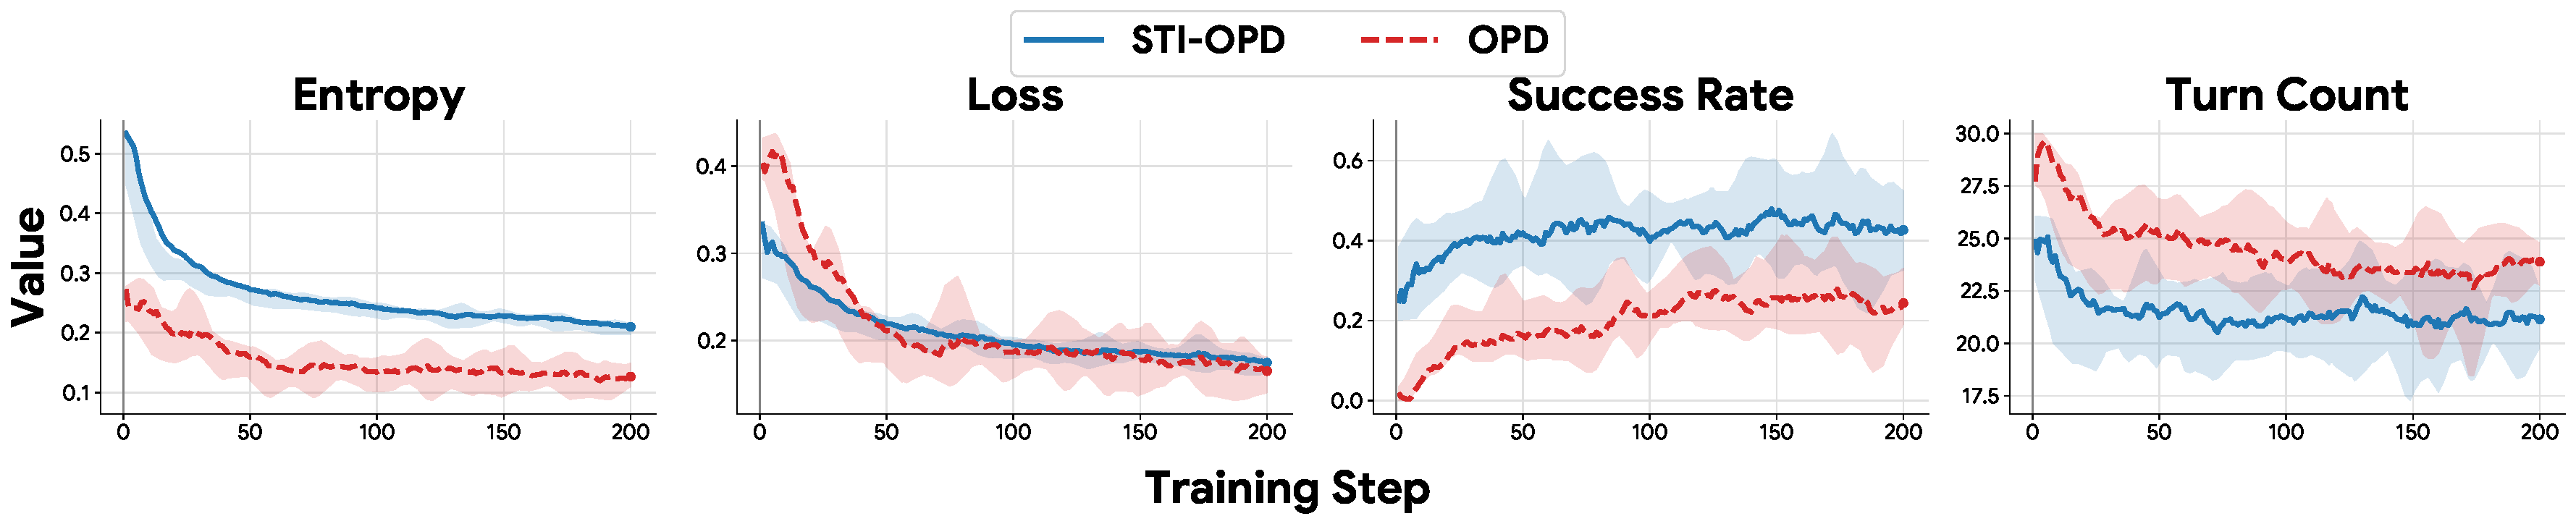
\includegraphics[width=1.\linewidth]{figs/training_dynamics.pdf}
    \caption{Training dynamics of \name and standard OPD on ALFWorld with Qwen3-1.7B as the student and Qwen3-4B as the teacher.}
    \label{fig:training_dynamics}
    \vspace{-1.0em}
\end{figure} 

\vspace{-0.5em}


\Cref{tab:ablation_study} isolates the contributions of the components in \name.
Replacing $k_3$ with $k_1$ reduces performance in both environments, supporting the use of a non-negative discrepancy estimator with lower variance near policy agreement for intervention.
We further compare the proposed stochastic intervention strategy against deterministic thresholding in \Cref{app:stochastic_vs_deterministic}. The stochastic strategy consistently performs better across ALFWorld and ScienceWorld without requiring a manually selected decision boundary.
Removing importance weighting causes the largest degradation on each reported task, highlighting the importance of correcting the sampling mismatch introduced by teacher-generated tokens.
Replacing reverse KL with forward KL also consistently reduces performance (we also study its impact on mitigating forgetting in \Cref{app:reverse_kl_forgetting}), favoring preservation of the conditional reverse-KL objective through importance weighting over changing the distillation objective.



\subsection{Mechanism, Scaling, and Cost Analysis of \name}
\label{sec:analysis}

\vspace{-0.5em}
\paragraph{Training Dynamics.}
As shown in \Cref{fig:training_dynamics}, \name achieves higher success rates early in training and maintains its advantage over standard OPD.
It also preserves higher policy entropy while requiring fewer interaction turns, suggesting greater policy diversity alongside more efficient task execution.
Although the training losses become similar at later stages, the success-rate gap persists, indicating that comparable distillation losses do not necessarily translate into comparable agentic performance.

\begin{figure}[t]
    \centering

    \begin{minipage}[t]{0.58\linewidth}
        \centering
        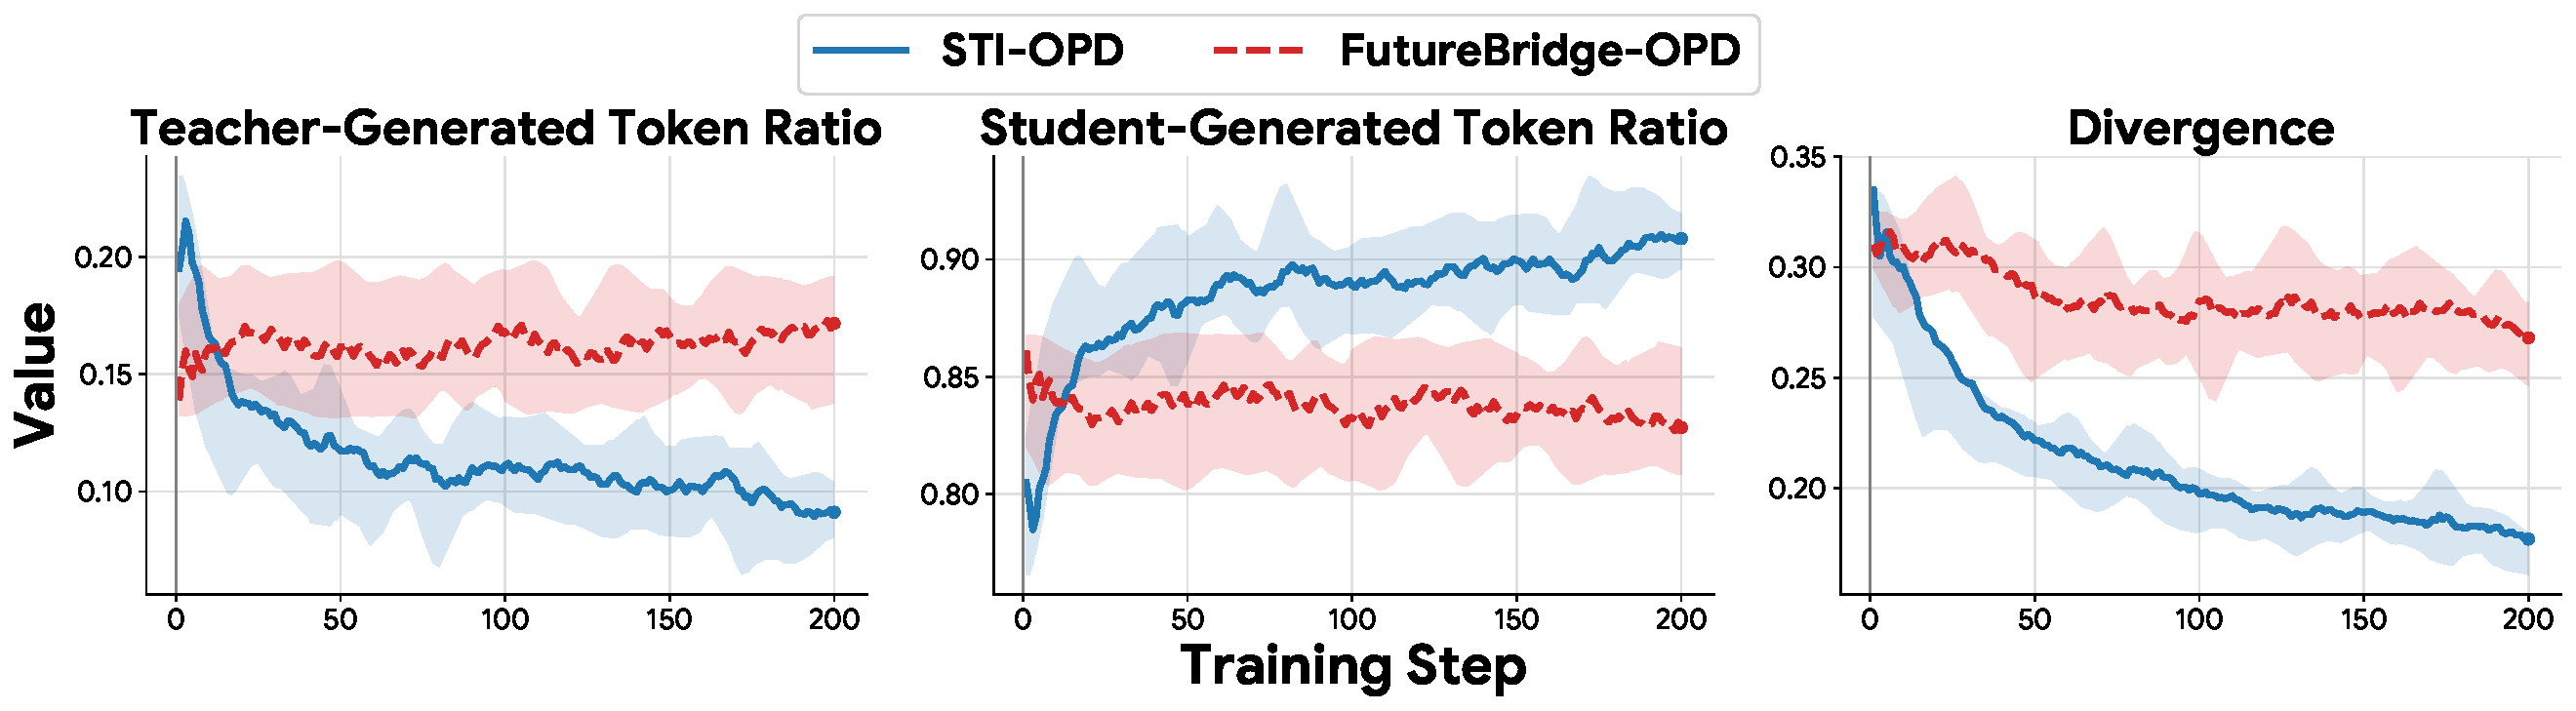
\includegraphics[width=\linewidth]{figs/sti_opd_dynamics.pdf}
        \caption{Intervention and policy discrepancy dynamics of \name and \textsc{FutureBridge-OPD} on ALFWorld, using Qwen3-1.7B as the student and Qwen3-4B as the teacher.}
        \label{fig:age_opd_dynamics}
    \end{minipage}
    \hfill
    \begin{minipage}[t]{0.4\linewidth}
        \centering
        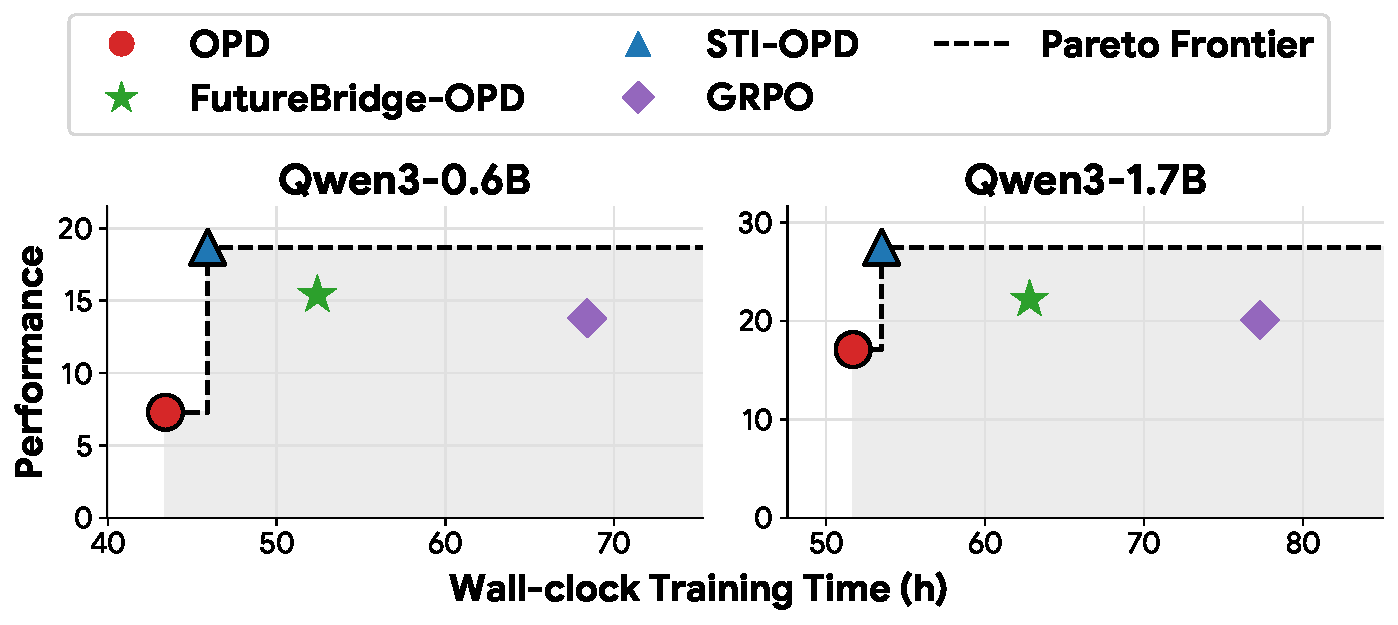
\includegraphics[width=\linewidth]{figs/wallclock_time_patero.pdf}
        \caption{Performance versus training wall-clock time. The dashed line indicates the empirical Pareto frontier. }
        \label{fig:wallclock_time}
    \end{minipage}

    \vspace{-1.0em}
\end{figure}


\vspace{-0.5em}
\paragraph{Mechanism Analysis.}
\Cref{fig:age_opd_dynamics} shows that \name shifts progressively from teacher-generated to student-generated tokens as training proceeds, and that the shift is more pronounced than for \textsc{FutureBridge-OPD}.
Alongside this shift, the teacher--student policy discrepancy decreases toward zero, as measured by the turn-level score in \Cref{eq:normalized_turn_score}.
These coupled trends are what the intervention rule prescribes: the teacher takes over more often when policy discrepancy is large, then cedes control as the student aligns.
Training therefore approaches the student-controlled regime used at inference time on its own, without a predefined intervention schedule.
\Cref{app:case_studies} shows cases and discussions about the mechanism of \name.

\vspace{-0.5em}
\paragraph{Scalability.}
Replacing the Qwen3-4B teacher with large-scale Qwen3-32B lifts each method accordingly. 
\name keeps the lead on each ALFWorld subtask and on ScienceWorld: with the 1.7B student it reaches $97.8$ on \textsc{Look} and $56.3$ on ScienceWorld, against $90.4$ and $46.2$ for \textsc{FutureBridge-OPD} (see details in \Cref{app:larger_teacher_results}).
The mechanism is therefore not specific to the Qwen3-4B teacher, and its margin does not close as the teacher grows.

\vspace{-0.5em}
\paragraph{Cost Analysis.}
\Cref{fig:wallclock_time} shows that \name lies on the empirical Pareto frontier at both student sizes.
\name improves substantially over standard OPD with modest additional training time. 
Compared with \textsc{FutureBridge-OPD}, \name achieves higher performance at lower computational cost. 
To further rule out the possibility that these gains arise simply from greater teacher usage, we additionally compare intervention-based methods under the same teacher-intervention budget in \Cref{app:teacher_computation_matched}.
\name remains consistently better under this matched budget, indicating that its advantage comes from more effective allocation and utilization of teacher guidance rather than simply more frequent teacher intervention.
Its efficiency relative to \textsc{FutureBridge-OPD} is consistent with estimating discrepancy from the existing student proposal without additional lookahead rollouts. 
Moreover, the intervention frequency of \name decreases as the student policy aligns with the teacher, further reducing teacher dependence over training. 
Compared with \textsc{GRPO}, \name's advantage lies in its lower rollout computational cost, because it does not require group rollouts for reward normalization.
Together, these results support a favorable performance--cost trade-off.
